\subsubsection{Curvature}

Differential geometry provides a scalar quantity\cite{Kuhnel2008} assignable to each point of a one-dimensional differntiable function, the \emph{curvature} $\kappa$.
This conecept can be generalized to higher dimensions and two common curvatures exist for surfaces in three-dimensional space, \gls{gaussian-curvature} and \gls{mean-curvature}.
\begin{figure}[H]
    \begin{subfigure}[t]{0.47\textwidth}
        \scalebox{0.9}{%
        \begin{tikzpicture}
\begin{axis}[xmin=-0.7,
             xmax=0.7,
             ymin=-0.1,
             ymax=1.1,
             samples=200,
             axis line style={draw=none},
             tick style={draw=none},
             xticklabels={\empty},
             yticklabels={\empty},
             grid=major,
             plot box ratio={2 1},
             axis equal]
    \draw[plotorange, line width=1.3pt] (axis cs:0,0.5) circle [radius=50];
    \addplot[plotblue, line width=1.5pt] {x*x};
    \coordinate (C) at (axis cs:{0.0,0.5});
    \coordinate (O) at (axis cs:{0.0,0.0});
    \coordinate (L) at (axis cs:{0.1,0.25});
    \node at (L) {$\mathbf{r}$};
    \node[label={90:{$\mathbf{C}$}},circle,fill,inner sep=1pt] at (C) {};
    \draw[thick,-](C)--(O);
\end{axis}
\end{tikzpicture}

        }
        \caption{The curvature of a line at a specific point is defined through its osculating circle.}\label{fig:osculating_circle}
    \end{subfigure}
    \begin{subfigure}[t]{0.47\textwidth}
        \scalebox{0.9}{%
        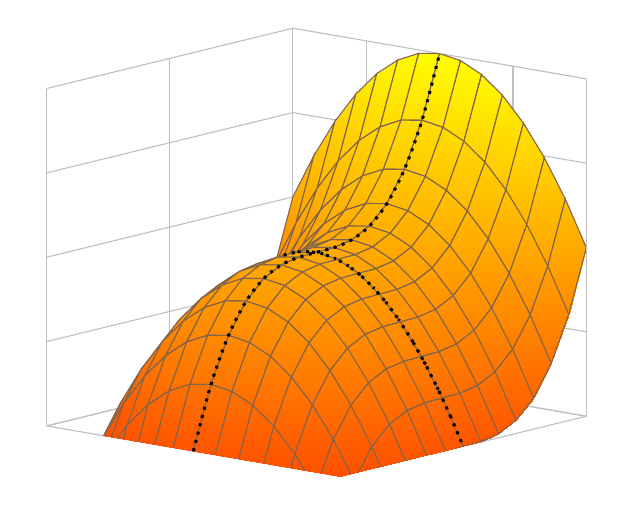
\begin{tikzpicture}
\begin{axis}[xmin=-1.0,xmax=1.0,
             ymin=-1.0,ymax=1.0,
             zmin=-1.0,zmax=1.0,
             grid=major,
             axis line style={draw=none},
             tick style={draw=none},
             view={310}{35},
             xticklabels={\empty},
             yticklabels={\empty},
             zticklabels={\empty},
             plot box ratio={1 1 3},
             colormap/redyellow]
\newcommand\func[2]{#1^3 - #2^2}
\definecolor{darkorange}{HTML}{84644B}

    \addplot3[surf,
              shader=faceted interp,
              faceted color={darkorange},
              samples=15,
              domain=-1:1,
              y domain=-1:1] {\func{x}{y}};

    % plot curve for x direction
    \addplot3[samples=15,
              domain=-1:1,
              samples y=1,
              dotted,
              black,
              line width=1.1pt,
              smooth] (x, 0, \func{x}{0});
    % plot curve for y direction
    \addplot3[samples=15,
              domain=-1:1,
              y domain=-1:0.22,
              dotted,
              black,
              line width=1.1pt,
              smooth] (0, y, \func{0}{y});
\end{axis}
\end{tikzpicture}

        }
        \caption[Visualization of curvature for curves and surfaces]{The curvature of a surface at a given point depends on the direction of measurement. The principal curvatures are the maximum and minimum value of curvatures in all directions.}\label{fig:curvature_surface}
    \end{subfigure}
    \caption[Curvature of Curves and Surfaces]{The curvature of a curve is defined through its osculating circle. This simple definition is not possible for surfaces in three dimensions. Each point on the surface does have a minimum and maximum curvature if analyzing all directions, the \emph{principal curvatures}.}
\end{figure}
A straight line has no curvature, hence $\kappa = 0$.
The curvature of a circle is defined is the inverse of its radius.
\begin{equation}
    \kappa_{circle} = \frac{1}{r}
\end{equation}
Any point's curvature on a one-dimensional, twice differentiable function is defined as the curvature of its osculating circle, visualized in Figure~\ref{fig:osculating_circle}.

The curvature of any point of a surface in three-dimensional space is ambigous, because it has infinite many curves crossing through this point.
But it exists a maximum and minimum curvature at this point, the \emph{principal curvatures} $k_1$ and $k_2$.
Figure~\ref{fig:curvature_surface} visualizes the minimum and maximum curvature of a surface in three-dimensional space as dotted black lines.
The \emph{\Gls{gaussian-curvature}} $\mathcal{K}$ is defined as the product
\[
    \mathcal{K} = k_1 k_2
\]
and the \emph{\Gls{mean-curvature}} $\mathcal{H}$ as the mean
\[
    \mathcal{H} = \frac{1}{2} (k_1 k_2)
\]
of the principal curvatures.

Both quantities can be calculated differently, as the curvature is related to the derivates of a function.
The range image is the two-dimensional function $f(u, v)$ and $f_u$, $f_v$, $f_{uu}$ and $f_{vv}$ its partial derivatives.
\begin{equation}
\begin{aligned}
    \mathcal{K} &= \frac{f_{uu} f_{vv} - f_{uv}^2}{{(1 + f_u^2 + f_v^2)}^2} \\
    \mathcal{H} &= \frac{{(1 + f_{v}^2)} f_{uu} - 2 f_u f_v f_{uv} + {(1 + f_u^2)} f_{vv}}{2 \sqrt{1 + f_u^2 + f_v^2}^3}
\end{aligned}
\end{equation}
The first and second derivatives can be approximated with $\mathcal{O}(\Delta x^2)$ accuracy.
\begin{align*}
    f_{x} &= \frac{y_{i+1} - y_{i-1}}{2 \Delta x} \\
    f_{xx} &= \frac{y_{i+1} + y_{i-1} - 2 y_{i}}{{\Delta x}^2}
\end{align*}

\begin{figure}[H]
    \begin{subfigure}[t]{0.32\textwidth}
        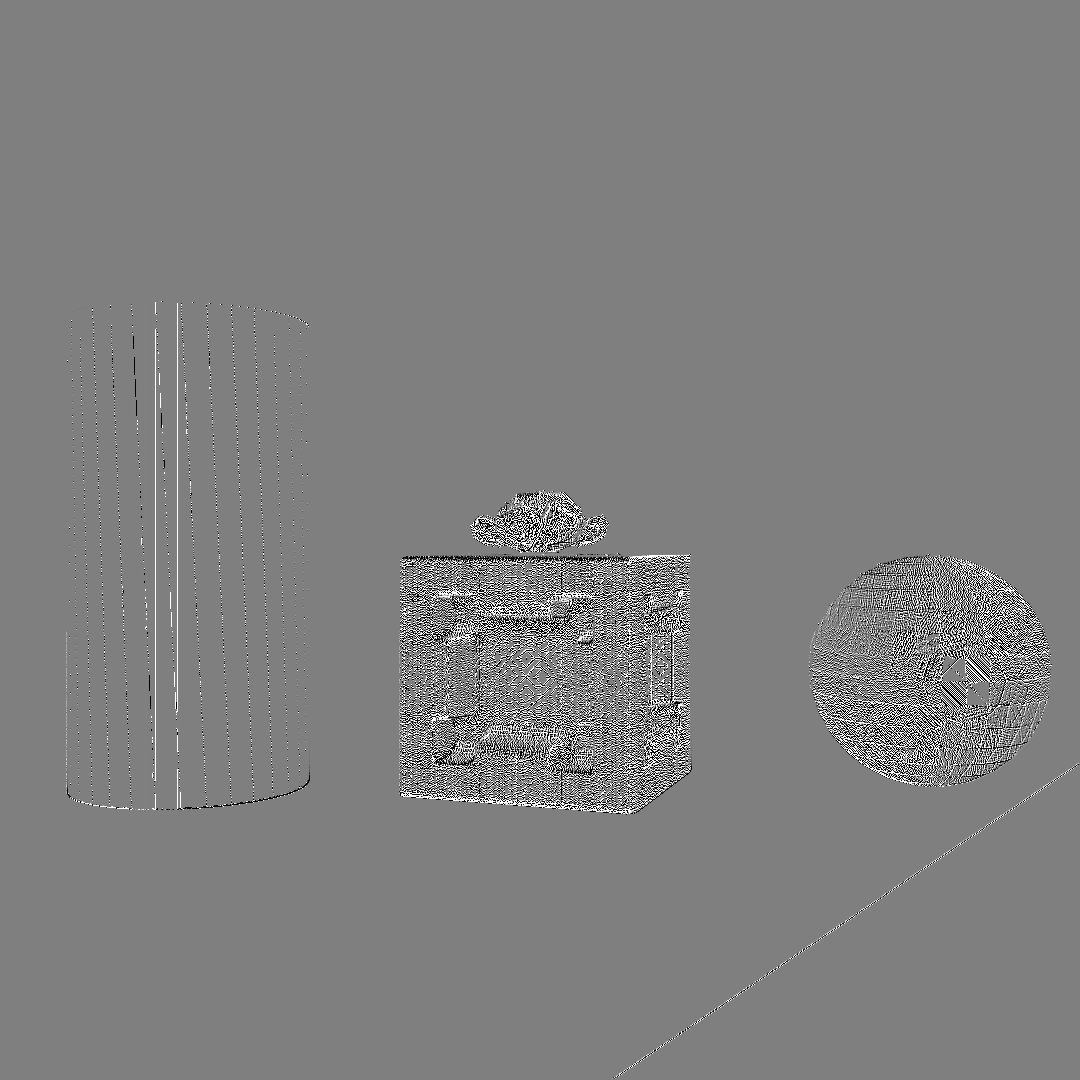
\includegraphics[width=\linewidth]{chapter04/img/mean-0001.png}
    \end{subfigure}
    \begin{subfigure}[t]{0.32\textwidth}
        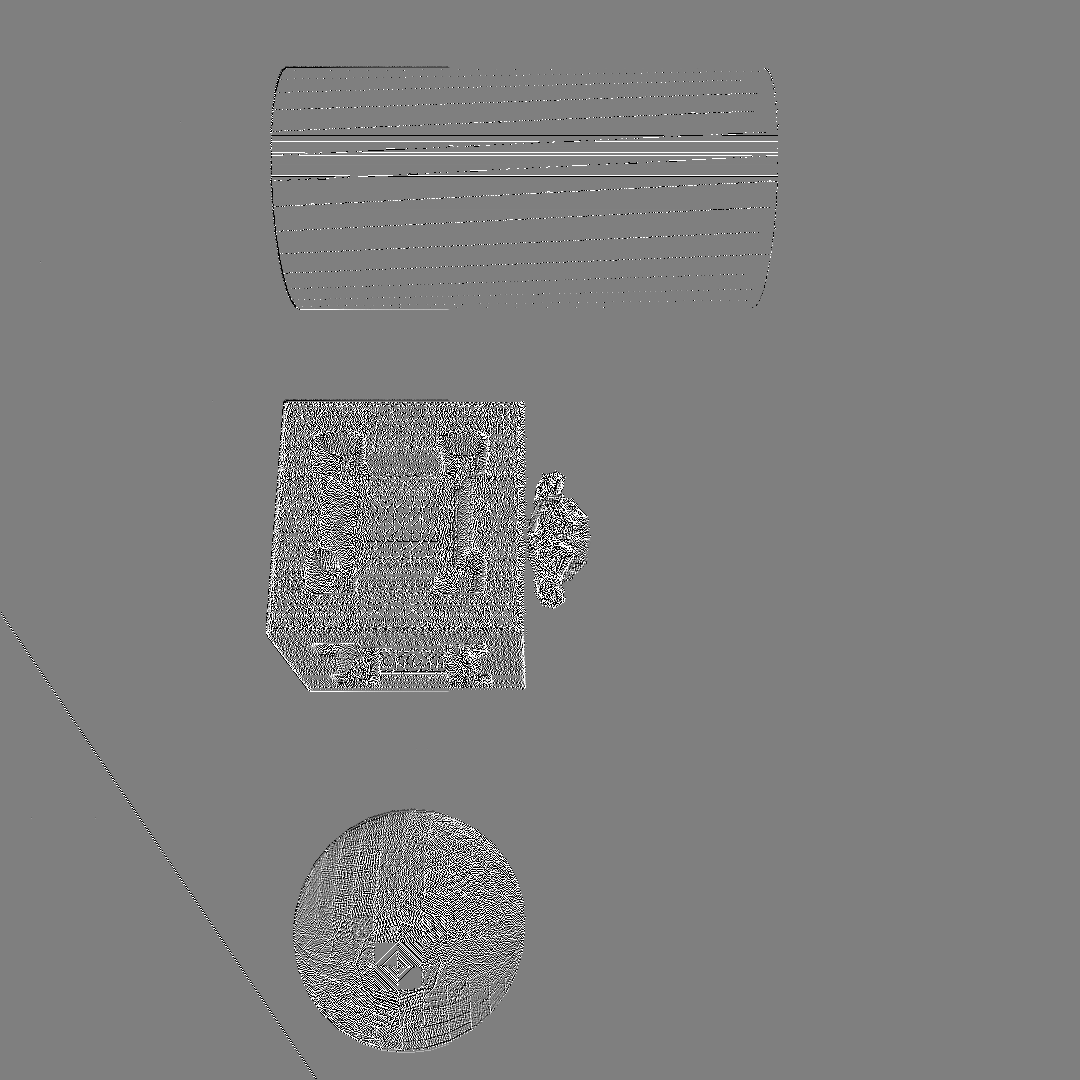
\includegraphics[width=\linewidth]{chapter04/img/mean-0030.png}
    \end{subfigure}
    \begin{subfigure}[t]{0.32\textwidth}
        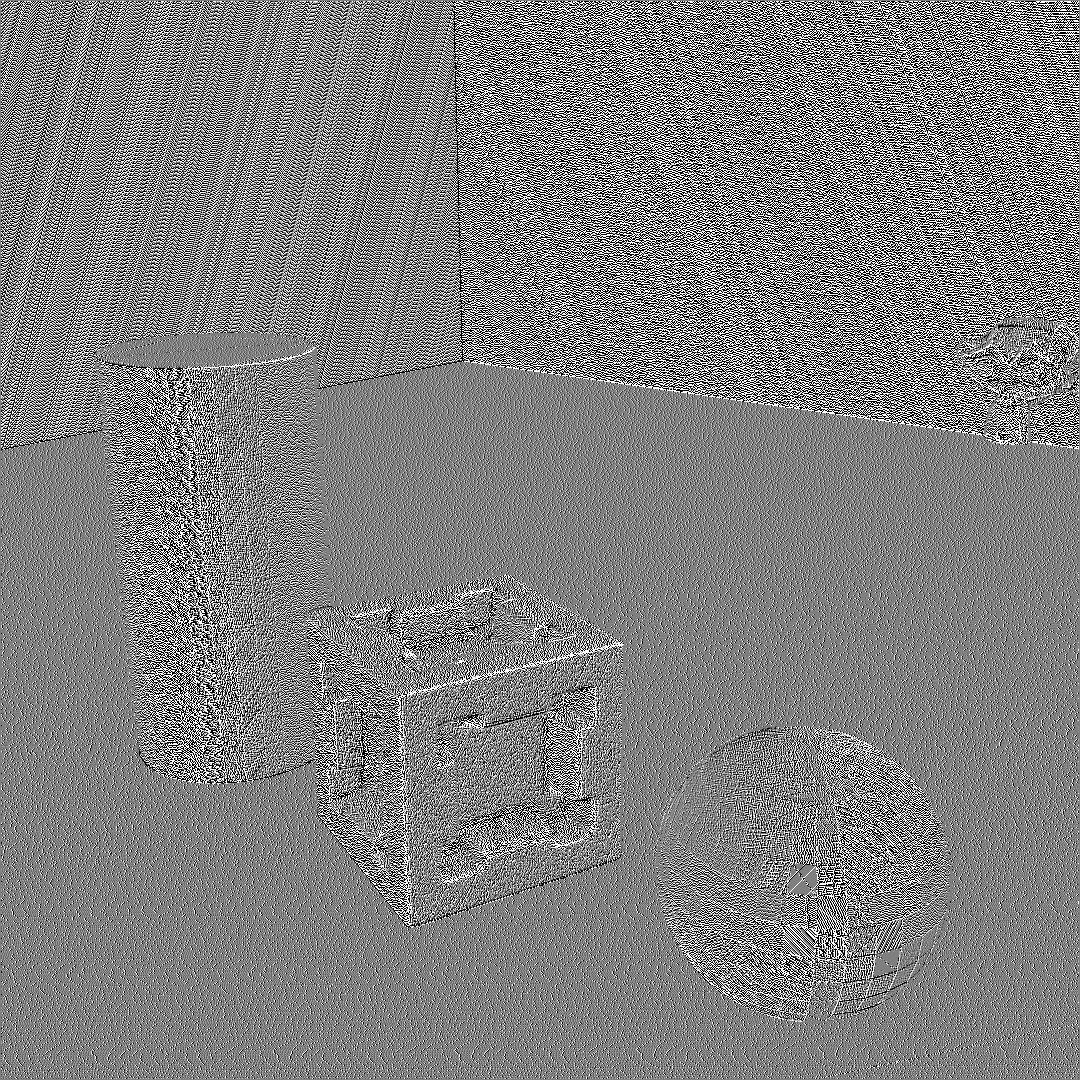
\includegraphics[width=\linewidth]{chapter04/img/mean-0210.png}
    \end{subfigure}
    \caption[\Gls{mean-curvature} in the synthetic scene]{The \Gls{mean-curvature} for the synthetic scene}\label{fig:mean-curvature}
\end{figure}
The result in Figure~\ref{fig:mean-curvature} is similar to the Multi-Directional bearing angle image.
The \gls{mean-curvature} is rotation invariant but the result is very unstable to noise.
Another limiting factor is the conversion to a integer based quantity.
Both the \gls{mean-curvature} and \gls{gaussian-curvature} are unbound and can take any real number.
Simple scaling between the computed minimum and maximum value is unstable between images and results in completly gray images as these quantities have noticable outliers.
As solution for this problem the computed values are clamped to a predefined range, for example $\mathcal{H},\mathcal{K} \in (-20, 20)$ and then scaled to the desired image depth of the feature image.

Figure~\ref{fig:gaussian-curvature} shows the images for the \gls{gaussian-curvature}.
It is even more prone to noise in the input and suffers from the same range issue.
\begin{figure}[H]
    \begin{subfigure}[t]{0.32\textwidth}
        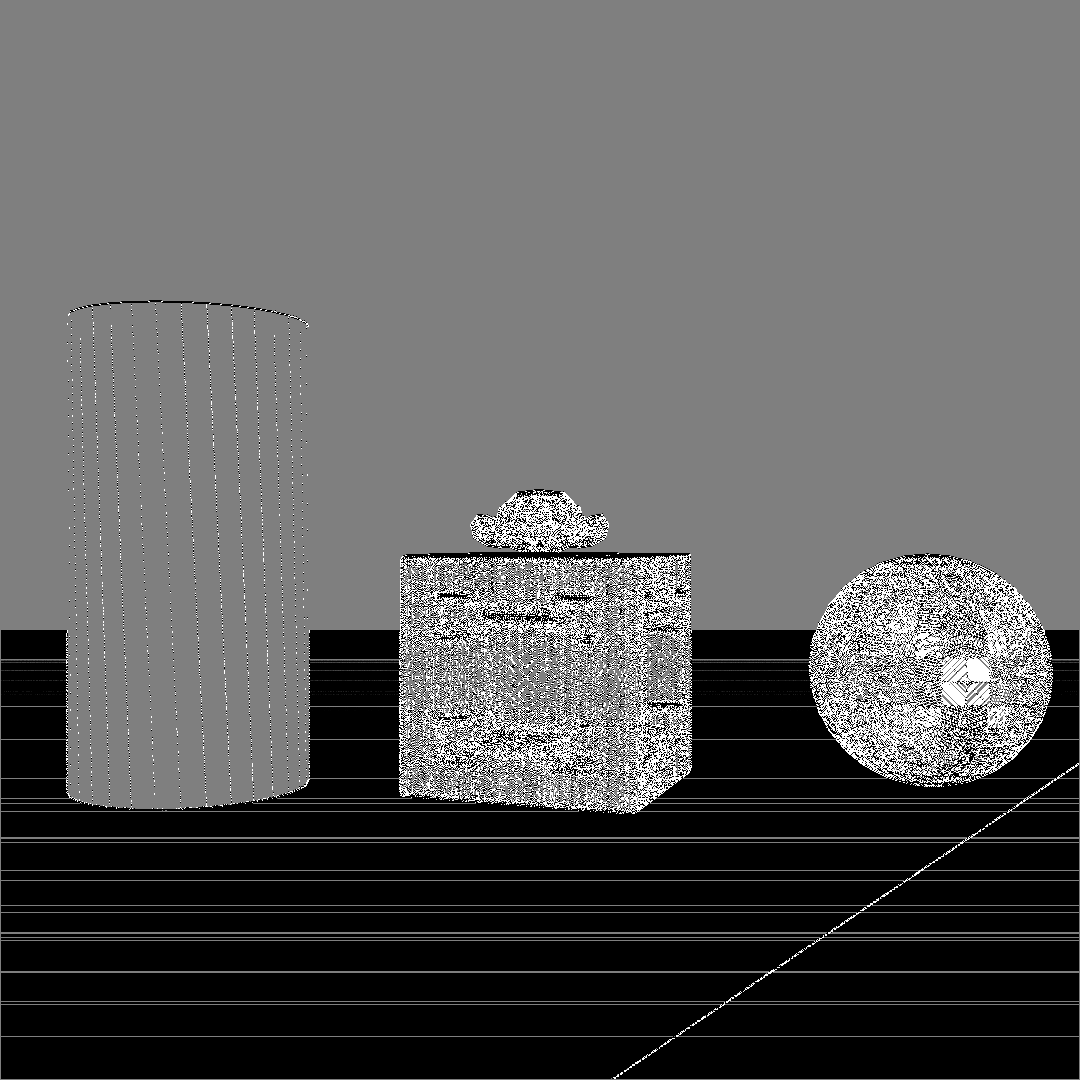
\includegraphics[width=\linewidth]{chapter04/img/gauss-0001.png}
    \end{subfigure}
    \begin{subfigure}[t]{0.32\textwidth}
        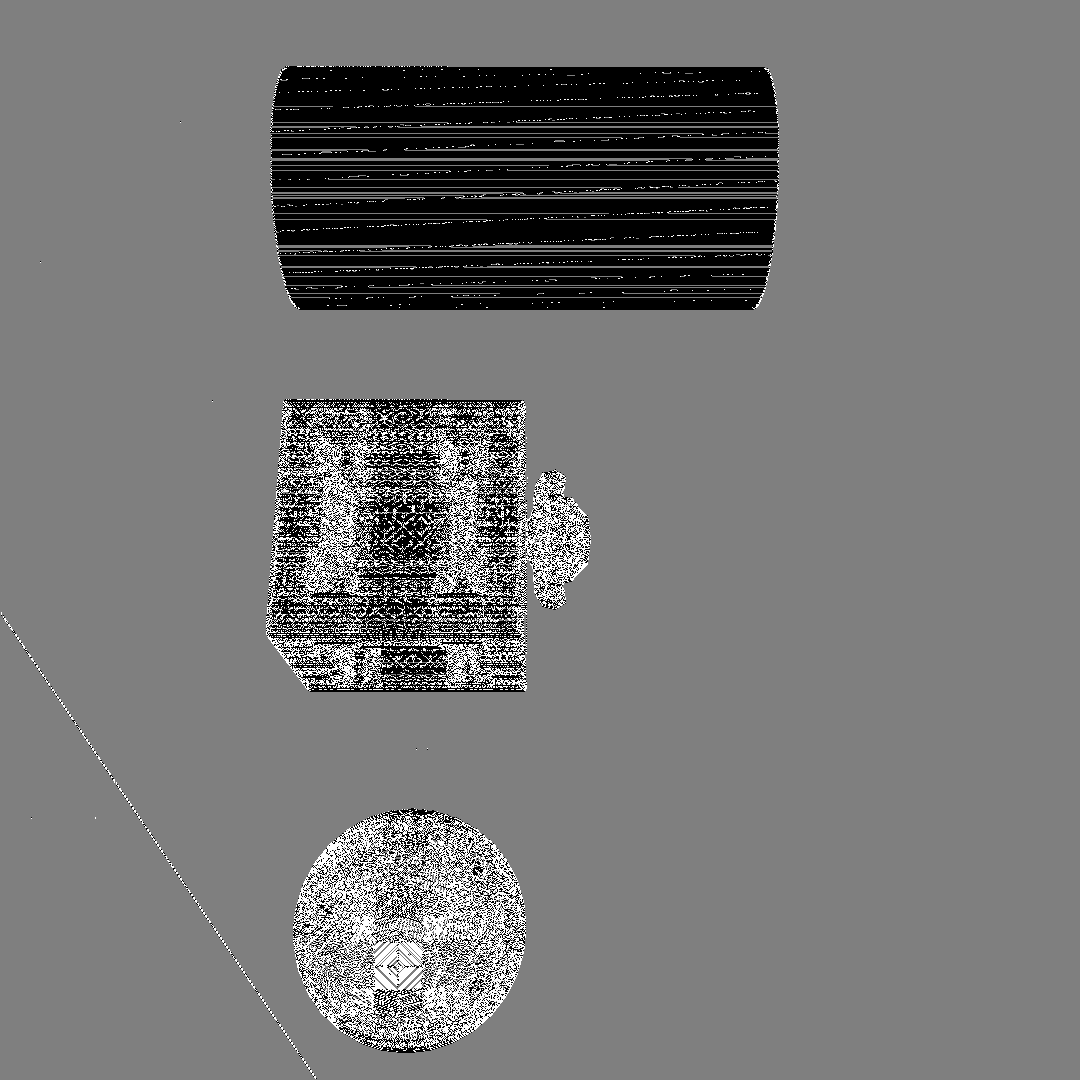
\includegraphics[width=\linewidth]{chapter04/img/gauss-0030.png}
    \end{subfigure}
    \begin{subfigure}[t]{0.32\textwidth}
        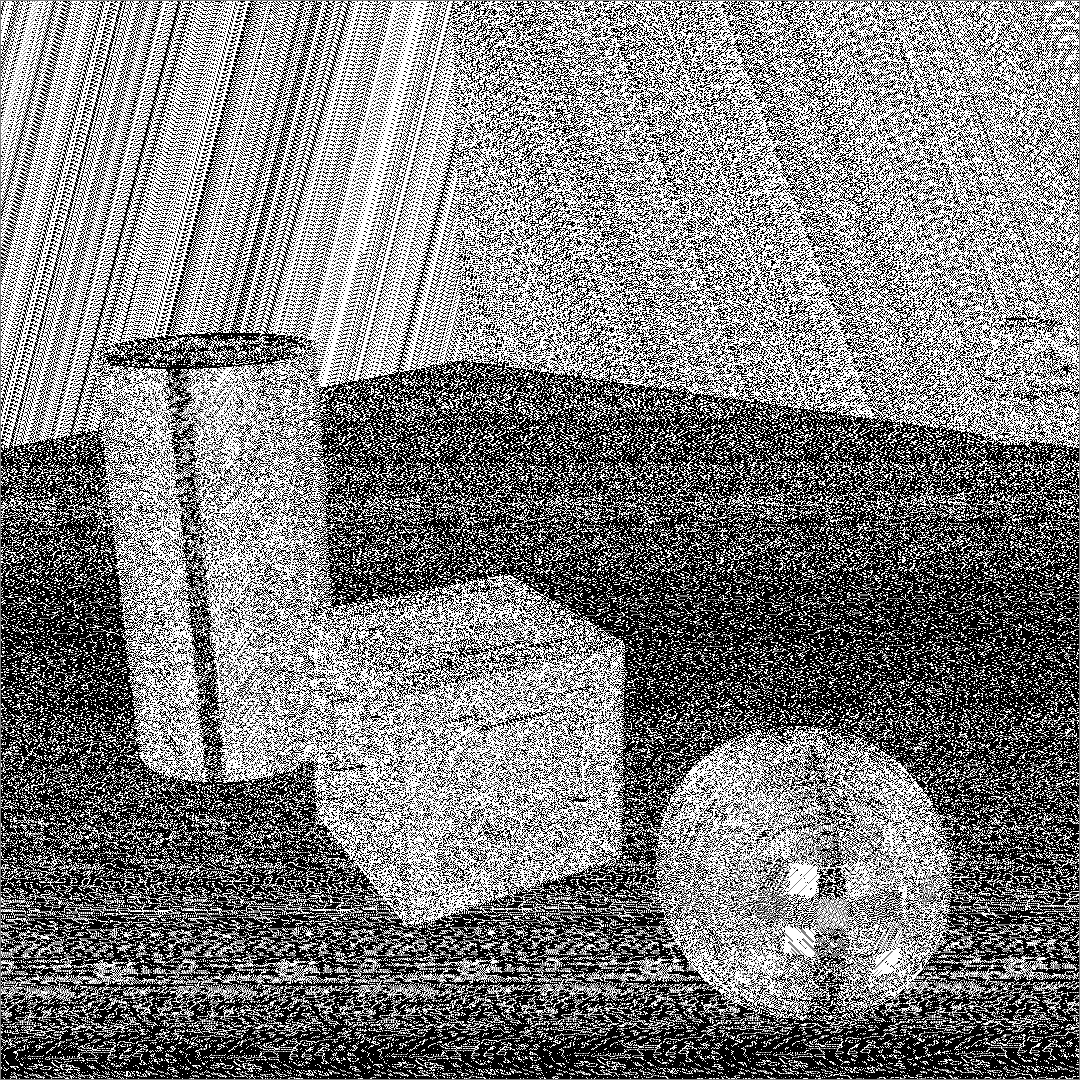
\includegraphics[width=\linewidth]{chapter04/img/gauss-0210.png}
    \end{subfigure}
    \caption[\Gls{gaussian-curvature} in the synthetic scene]{The \Gls{gaussian-curvature} for the synthetic scene}\label{fig:gaussian-curvature}
\end{figure}
Computing the curvature for the whole image has the theoretical weakness for discontinuities at object boundaries.
For perfect depth sensing the derivatives do not exist at these points.
A mathematically optimal computation requires object identification or meshing of the scene.
Such a requirement seems unreasonable for a foundational processing step in potential real-time use cases.
